\section{Project Planning and Timeline}
The overall project will span a total of two academic semesters of the senior year (a total of approximately 8 months) and will comprise a set of goals for each semester. The project will be managed using an agile methodology, where by the end of the project, two deliverables will be obtained: MVP1 and MVP2. This section will break down the project planning and timeline for only MVP2, as well as expected deliverables for each phase.

\subsection{Channels}
Throughout the project, two essential tools will be used to facilitate communication and task delegation within the project. The first tool is Discord, a multi-functional communication tool that is practical for meetings, scheduling events, and so on. Discord will be used as the primary communication tool for the members in the project, as well as for some advisors. The second tool is Jira, an agile project management tool that facilitates task delegation and software project management. Jira will be used to track the tasks of each member in the project, as well as to track software features and bugs within the project in the form of tickets for ease of audit. Additionally, it will also comprise the customer journey of each feature of the robot in the form of “user stories.”

\subsection{MVP 2 - Non-Commercial Prototype}
MVP 2 will span the entirety of academic semester 2 (from January until April) and will focus on implementing a non-commercial prototype. To elaborate, the team expects a prototype that is viable for testing, but does not consider factors such as security, quality testing, etc to a deep level. MVP 2 will consist of four sprints, each focusing on distinct milestones. Sprint 0, spanning Weeks 1–3, will focus on initial planning, including project scope definition, task delegation, parts acquisition, and 3D-printed CAD designs for components such as the head, arms, base, and outer shell. Experimentation with the Jetson Nano will include configuring the LCD screen, integrating code, and setting up motor interfacing. Preliminary research on Bayesian networks will also be conducted, culminating in a raw prototype. Sprint 1, lasting from Week 4 to Week 7, will focus on assembling a functional prototype and implementing at least four of the planned 15 action bubbles, including greetings, subtle robot movements, positive reinforcement for happiness, and stress-response actions. Debugging and fine-tuning will also take place during this phase. Sprint 2, spanning Weeks 9–12, will prioritize completing all 15 action bubbles, engaging with potential end-user testing candidates, and preparing for iterative testing. Sprint 3, covering Weeks 13–16, will emphasize team testing, quality assurance, and two rounds of end-user testing in Weeks 14 and 15, followed by preparation for the final presentation. By the end of MVP 2, the project will deliver an integrated prototype that successfully combines hardware and software, validated through comprehensive team and end-user testing, establishing a strong foundation for future development.

\begin{figure}[!ht]
      \centering
      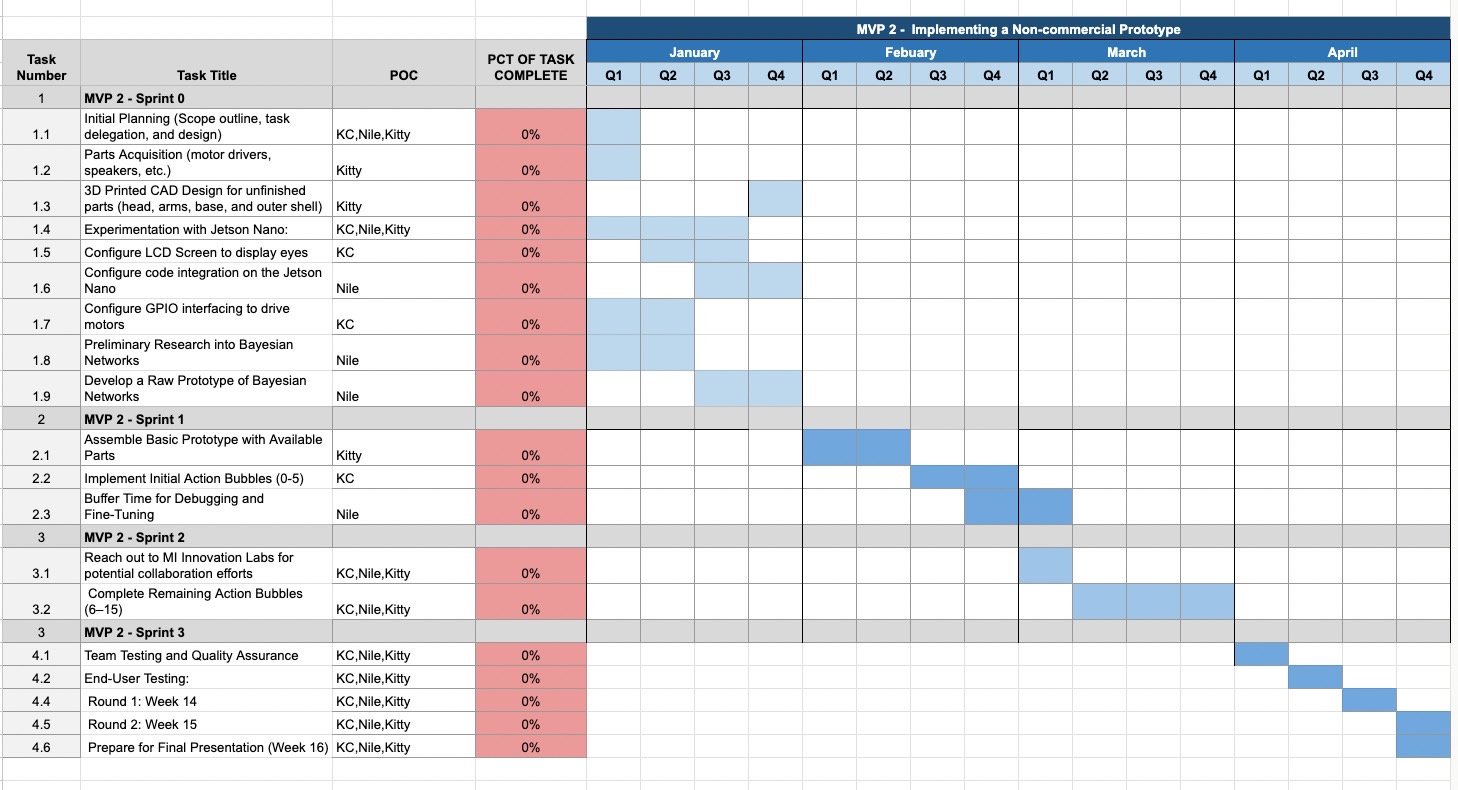
\includegraphics[width=0.9\textwidth]{gantt.jpg}
      \caption{Project GANTT Chart for MVP 2}
      \label{fig:gantt}
\end{figure}

\begin{enumerate}
\item\textbf{MVP 1 - Sprint 0 (Weeks 1–3)}

\subitem \textit{1.1} Initial Planning (Scope outline, task delegation, and design)
\subitem \textit{1.2} Parts Acquisition (motor drivers, speakers, etc.)
\subitem \textit{1.3} 3D Printed CAD Design for unfinished parts (head, arms, base, and outer shell)
\subitem \textit{1.4} Experimentation with Jetson Nano:
      \subsubitem \textit{1.4.1} Configure LCD Screen to display eyes
      \subsubitem \textit{1.4.2} Configure code integration on the Jetson Nano
      \subsubitem \textit{1.4.3} Configure GPIO interfacing to drive motors
\subitem \textit{1.5} Preliminary Research into Bayesian Networks
\subitem \textit{1.6} Develop a Raw Prototype of Bayesian Networks 

\item \textbf{MVP 1 - Sprint 1 (Weeks 3–7)}
\subitem \textit{2.1} Assemble Basic Prototype with Available Parts
\subitem \textit{2.2} Implement Initial Action Bubbles (0-5)
\subitem \textit{2.3} Buffer Time for Debugging and Fine-Tuning

\item \textbf{MVP 1 - Sprint 2 (Weeks 9–12)}
\subitem \textit{3.1} Reach out to MI Innovation Labs for potential collaboration efforts
\subitem \textit{3.2} Complete Remaining Action Bubbles (6–15)

\item \textbf{MVP 1 - Sprint 3 (Weeks 13–16)}
\subitem \textit{4.1} Team Testing and Quality Assurance
\subitem \textit{4.2} End-User Testing:
     \subsubitem \textit{4.2.1} Round 1: Week 14
     \subsubitem \textit{4.2.2} Round 2: Week 15
\subitem \textit{4.3} Prepare for Final Presentation (Week 16)
\end{enumerate}

\subsection{Current Progress and Challenges}
In terms of current progress, the robot is still in its early development. Throughout the last semester, the team focused on project concept development and software architecture, where the hardware components were only considered nearing the end of the semester. As such, the main challenge is configuring the hardware components to work correctly, where the main concern currently is the LCD screen that represents the eyes. Currently, the eyes of the robot used a Python library called OpenCV, which is an image processing library allowing the drawing of various shapes. The eyes were hard coded as various shapes and patterns drawn on a black canvas, as shown in Figure \ref{fig:eye}. The main challenge with this approach was the scalability and implementation time. Since each frame is hard coded, it does not allow for much flexibility and complex shapes. However, the upside is that it can easily be built in as a class into the main code. 

\begin{figure}[ht]
      \centering
      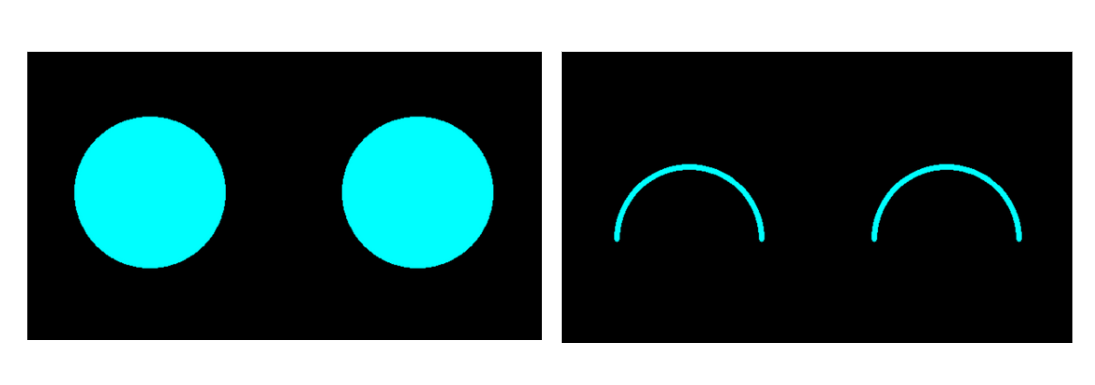
\includegraphics[width=\textwidth]{eye.png}
      \caption{OpenCV Eyes Example for “Happy”}
      \label{fig:eye}
\end{figure}

The team has not yet finalized the approach to displaying the eyes on the screen, deciding between OpenCV shapes like in semester 1, or to use a more conventional method like using game frames. Additionally, the system has not been migrated or tested on the Jetson Nano, which will be the main processor for the project. As such, unprecedented challenges such as incompatibility may be faced later. In response to this, the team has allocated buffer time to each sprint to ensure a feasible outcome.

Another key challenge is defining the “action bubbles”. These action bubbles indicate the set of all predefined interactions the robot may have with the user. For instance, an action bubble may include the robot’s eyes changing color and shape to resemble a wink, one of its arms raised up, and its head tilting a little bit, to form a “greetings!” action bubble. The team must not only implement these, but also define the objectives of these actions so that they have an actual positive impact on the user. These actions will be finalized after a feedback loop in the testing phase. 

Additionally, significant progress has been made on the software side, particularly with the development of the FER (facial emotion recognition) and SER (speech emotion recognition) systems. These systems are integral to the robot’s ability to understand and respond to the user’s emotional state. More details on the methodologies, implementation, and technical challenges of these systems will be addressed in the next section, \textit{Theory and Technical Backup}.